\documentclass[DM,authoryear,toc]{lsstdoc}
% lsstdoc documentation: https://lsst-texmf.lsst.io/lsstdoc.html
\input{meta}

% Package imports go here.
\usepackage{listings}
\usepackage{color}

\definecolor{dkgreen}{rgb}{0,0.6,0}
\definecolor{gray}{rgb}{0.5,0.5,0.5}
\definecolor{mauve}{rgb}{0.58,0,0.82}

\newenvironment{allintypewriter}{\ttfamily}{\par}

\lstset{frame=tb,
  language=SQL,
  aboveskip=3mm,
  belowskip=3mm,
  showstringspaces=false,
  columns=flexible,
  basicstyle={\small\ttfamily},
  numbers=none,
  numberstyle=\tiny\color{gray},
  keywordstyle=\color{blue},
  commentstyle=\color{dkgreen},
  stringstyle=\color{mauve},
  breaklines=true,
  breakatwhitespace=true,
  tabsize=3
}


% Local commands go here.

%If you want glossaries
%\input{aglossary.tex}
%\makeglossaries

\title{Validation Tests of the DP0.1 TAPserver on IDF}

% Optional subtitle
% \setDocSubtitle{A subtitle}

\author{%
Douglas L.\ Tucker
}

\setDocRef{RTN-026}
\setDocUpstreamLocation{\url{https://github.com/lsst/rtn-026}}

\date{\vcsDate}

% Optional: name of the document's curator
% \setDocCurator{The Curator of this Document}

\setDocAbstract{%
DP0.1 contains the DWF data set from the Vera C. Rubin LSST DESC DR2.
This data set contains, among other material, images and catalogs for
c.\ 300 sq deg of contiguous sky within the LSST footprint.  Here, we
present verfication tests of the catalog data contained within the
DP0.1 TAPserver on the Interim Data Facility (IDF).
}

% Change history defined here.
% Order: oldest first.
% Fields: VERSION, DATE, DESCRIPTION, OWNER NAME.
% See LPM-51 for version number policy.
\setDocChangeRecord{%
  \addtohist{1}{YYYY-MM-DD}{Unreleased.}{Douglas Tucker}
}


\begin{document}

% Create the title page.
\maketitle
% Frequently for a technote we do not want a title page  uncomment this to remove the title page and changelog.
% use \mkshorttitle to remove the extra pages

% ADD CONTENT HERE
% You can also use the \input command to include several content files.

\section{Introduction} \label{sec:intro}

This Rubin Technical Note (RTN-026) documents the validation of the
TAP service (Qserv) database on the Interim Data Facility (IDF) for
DP0.1.  DP0.1 contains the DWF data set from the Vera C.\ Rubin LSST
DESC Data Challege 2 (DC2).
%; \citep{2021ApJS..253...31L,2021arXiv210104855L}).
This data set contains, among other material, images and catalogs for
c.\ 300 sq deg of contiguous sky within the LSST footprint.  DP0.1 was
released to the

Here, we present verfication tests of the catalog data
contained within the DP0.1 TAPserver on the Interim Data Facility
(IDF).

DP0 is described in \citeds{RTN-001}.

DP0.1 was fully uploaded to the IDF by the end of March 2021.  It became
available to the the initial group of DP0 Delegates at the end of June 2021.

Initial DP0.2 re-processing of two tracts to a 1.5-year depth became
available for testing in the second half of October 2021.

Here, we generally used the TAP service to access Qserv via the Jupyter
notebooks running on the Rubin Science Platform (RSP) on the IDF,
although we occaionally used the NVO TOPCAT java software for initial
tests.  Access via the Jupyter notebook interface was achieved via the
following code:


\lstset{language=Python}
\begin{lstlisting}
# Import the Rubin TAP service utilities
from rubin_jupyter_utils.lab.notebook import get_tap_service, retrieve_query, get_catalog
# Get an instance of the TAP service
service = get_tap_service()
assert service is not None
assert service.baseurl == "https://data.lsst.cloud/api/tap"
\end{lstlisting}



\section{Basic Tests of the \texttt{dp01\_dc2\_catalalogs} Schema} \label{sec:basic}

As a first basic test of the DP0.1 contents of Qserv, we looked at which tables were available in the
\texttt{dp01\_dc2\_catalogs} schema:

\lstset{language=Python}
\begin{lstlisting}
%%time
now0=datetime.now()
schema_name = 'dp01_dc2_catalogs'
query = """SELECT table_name FROM TAP_SCHEMA.tables WHERE schema_name=%s""" % ("\'"+schema_name+"\'")
print(query)
results = service.search(query)
df = results.to_table().to_pandas()
table_full_name_list = df['table_name'].tolist()
print(table_full_name_list)
\end{lstlisting}

Here are the results, which match expectations:

\lstset{language=Python}
\begin{lstlisting}
SELECT table_name FROM TAP_SCHEMA.tables WHERE schema_name='dp01_dc2_catalogs'
['dp01_dc2_catalogs.forced_photometry', 'dp01_dc2_catalogs.object', 'dp01_dc2_catalogs.position', 'dp01_dc2_catalogs.reference', 'dp01_dc2_catalogs.truth_match']
CPU times: user 17 ms, sys: 0 ns, total: 17 ms
yWall time: 60.7 ms
\end{lstlisting}


Once we we checked that the above tables were, in fact, in the IDF Qserv database, our next simple test was to check how many entries (rows) there were in these 5 tables: 


\lstset{language=Python}
\begin{lstlisting}
for table in ['forced_photometry', 'object', 'position', 'reference', 'truth_match']:
   query = """SELECT count(*) FROM dp01_dc2_catalogs.%s""" % (table)
   print(query)
   results = service.search(query)
   df = results.to_table().to_pandas()
   count = df['count'].iloc[0]
   print(count)
   print("")
\end{lstlisting}

These are the results.

\lstset{language=SQL}
\begin{lstlisting}
SELECT count(*) FROM dp01_dc2_catalogs.forced_photometry
147088445

SELECT count(*) FROM dp01_dc2_catalogs.object
147088478

SELECT count(*) FROM dp01_dc2_catalogs.position
147088445
 
SELECT count(*) FROM dp01_dc2_catalogs.reference
147088445

SELECT count(*) FROM dp01_dc2_catalogs.truth_match
765823615
\end{lstlisting}

As expected, the \texttt{forced\_photometry}, \texttt{object}, \texttt{}, and \texttt{reference} tables have a (nearly) identical number of rows, since each of these tables refers to individual objects that are the same for all four of these tables.  (It has been noted that the \texttt{object} table contains 33 more rows than the other three of these 4 tables, but why this is so has yet to be fully investigated.)  The \texttt{truth\_match} has $\approx$5$\times$ as many entries as the other four catalogs.  A quick check indicates that  \texttt{truth\_match} contains a considerable number of objects with no match in (say) the \texttt{object} table, and the peak of \texttt{r\_mag} for entries in the \texttt{truth\_match} is $\sim$29.0 instead of $\sim$26.0 as it is for the texttt{object} table.

\section{More Detailed Tests of Individual Tables in the  \texttt{dp01\_dc2\_catalalogs} Schema} \label{sec:detailed}

A separate Jupyter notebook was created to test the contents of each
table in the \texttt{dp01\_dc2\_catalalogs} schema.  In each case,
similar steps were followed:
\begin{enumerate}
\item Import a set of standard python modules (\texttt{numpy},
  \texttt{pandas}, etc.) as well the Rubin TAP service utilities.
\item Get an instance of the TAP service at
  \url{https://data.lsst.cloud/api/tap}.
\item Verify the counts of entries for the table as was done in the
  general schema tests (Section~\ref{sec:basic}).
\item Verify the list of tracts as also was done in the general schema
  tests (Section~\ref{sec:basic}).
\item Loop over each tract:
  \begin{enumerate}
  \item Query for the full contents of the table for that tract (via asynchronous TAP query).
  \item Load the results of the query in a Pandas data frame.
  \item For each column in the Pandas data frame:
    \begin{enumerate}
    \item Count the total number of entries and the number of entries with a value of \texttt{NaN}.
    \item Calculate the 1\%-ile, the 50\%-ile (median), and the 99\%-ile value for that column via the Pandas \texttt{Series.quantile} function.
    \end{enumerate}
  \end{enumerate}
\item Once the the above statistics were measured for each column in each tract, the histogram over all the tracts for each column was plotted.
\item Once all was completed for the table being checked, the asynchronous TAP jobs could be deleted.
\end{enumerate}

Details of this process can be viewed in the rendered Jupyter notebooks at
\url{https://github.com/lsst/rtn-026/blob/master/notebooks/}.


Note, the process of querying a table for all its entries tract-by-tract and downloading to a Pandas data frame is very resource- and time-intensive.  Typically, the process to analyze a single table would take $\gtrsim$16 hours of wall clock time.  In fact, this was not possible for the larger table, \texttt{forced\_photometry} and a different, more approximate method had to be employed.


\lstset{language=Python}
\begin{lstlisting}
%%time
now0=datetime.now()
# `tract` is not a column in forced_photometry; so we need to be a little tricky...
query = """SELECT DISTINCT obj.tract 
           FROM %s.object as obj
           JOIN %s as x
           ON obj.objectId = x.objectId  
           ORDER BY obj.tract""" % \
        (schema_name, table_full_name)
print(query)
results = service.search(query)
df = results.to_table().to_pandas()
tract_list = df['tract'].tolist()
now1=datetime.now()
print("Total time:", now1-now0)
print(tract_list)
\end{lstlisting}


%\begin{allintypewriter}
\lstset{language=sh}
\begin{lstlisting}
SELECT DISTINCT obj.tract 
           FROM dp01_dc2_catalogs.object as obj
           JOIN dp01_dc2_catalogs.position as x
           ON obj.objectId = x.objectId  
           ORDER BY obj.tract
Total time: 0:01:53.352097
[2723, 2724, 2725, 2726, 2727, 2728, 2729, 2730, 2731, 2732, 2733, 2734, 2735, 2896, 2897, 2898, 2899, 2900, 2901, 2902, 2903, 2904, 2905, 2906, 2907, 2908, 3074, 3075, 3076, 3077, 3078, 3079, 3080, 3081, 3082, 3083, 3084, 3085, 3086, 3256, 3257, 3258, 3259, 3260, 3261, 3262, 3263, 3264, 3265, 3266, 3267, 3268, 3441, 3442, 3443, 3444, 3445, 3446, 3447, 3448, 3449, 3450, 3451, 3452, 3453, 3454, 3631, 3632, 3633, 3634, 3635, 3636, 3637, 3638, 3639, 3640, 3641, 3642, 3643, 3825, 3826, 3827, 3828, 3829, 3830, 3831, 3832, 3833, 3834, 3835, 3836, 3837, 4022, 4023, 4024, 4025, 4026, 4027, 4028, 4029, 4030, 4031, 4032, 4033, 4034, 4035, 4224, 4225, 4226, 4227, 4228, 4229, 4230, 4231, 4232, 4233, 4234, 4235, 4236, 4429, 4430, 4431, 4432, 4433, 4434, 4435, 4436, 4437, 4438, 4439, 4440, 4441, 4636, 4637, 4638, 4639, 4640, 4641, 4642, 4643, 4644, 4645, 4646, 4647, 4648, 4850, 4851, 4852, 4853, 4854, 4855, 4856, 4857, 4858, 4859, 4860, 5065, 5066, 5067, 5068, 5069, 5070, 5071, 5072, 5073, 5074]
CPU times: user 12.5 ms, sys: 3.93 ms, total: 16.4 ms
Wall time: 1min 53s
\end{lstlisting}
%\end{allintypewriter}



\subsection{\texttt{object} Table} \label{sec:object}

\begin{figure*}[h]
\centering
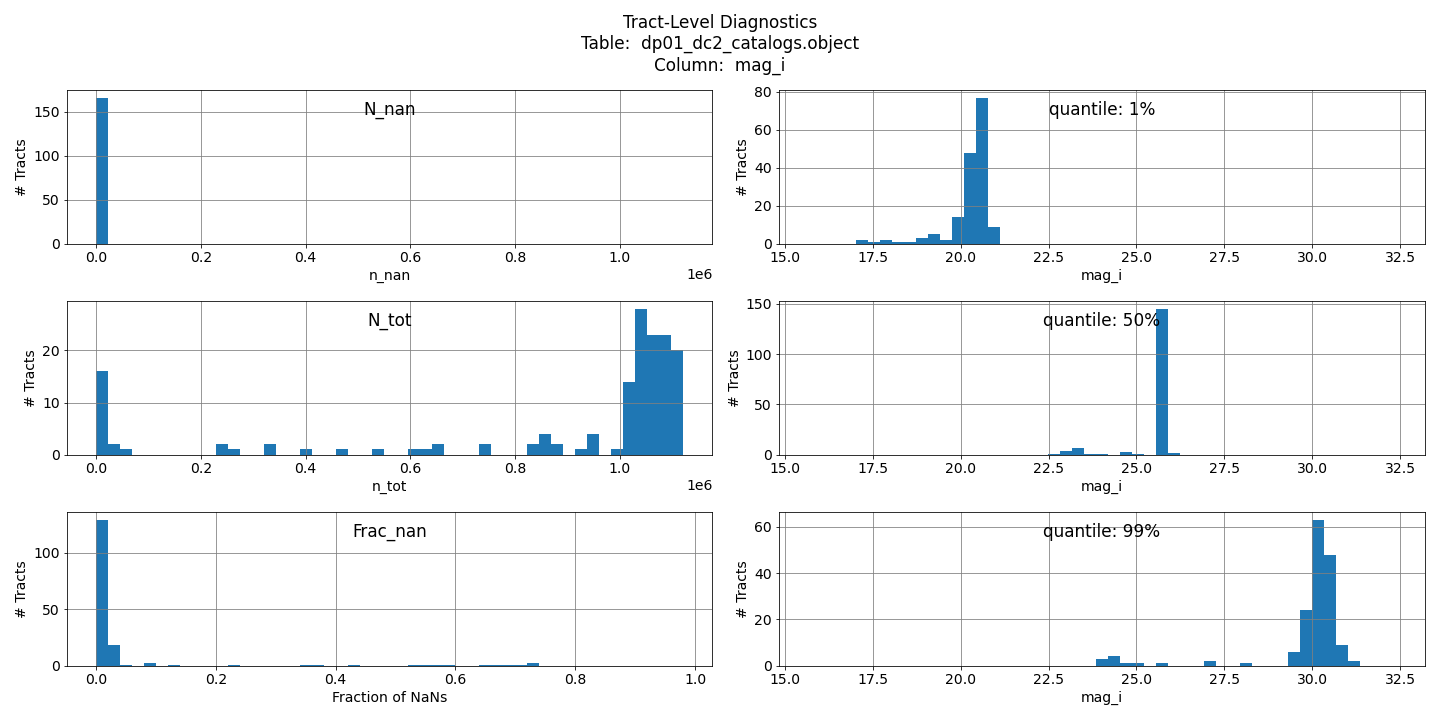
\includegraphics[width=1.0\linewidth]{Plots/TAP_verify_DP01.dp01_dc2_catalogs.object.mag_i.png}
\caption{}
\label{fig:object_mag_i}
\end{figure*}

\begin{figure*}[h]
\centering
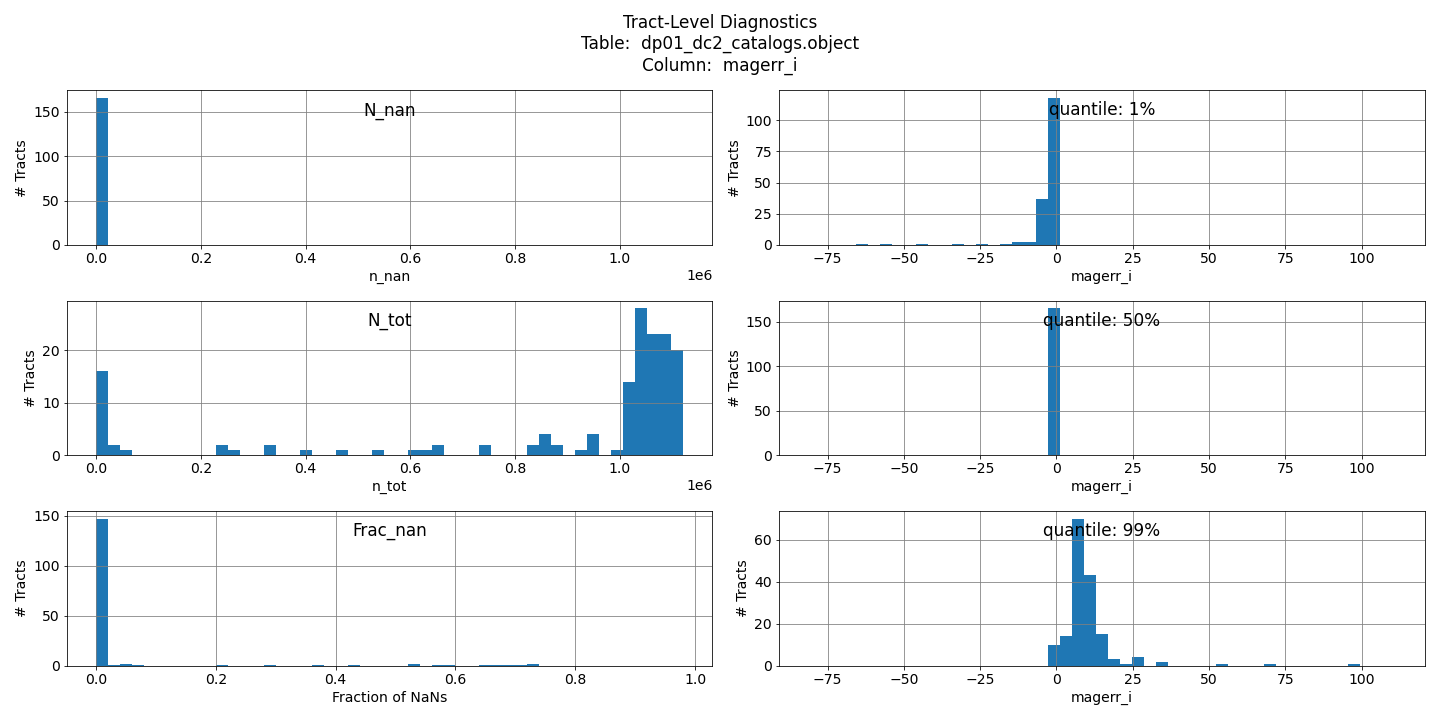
\includegraphics[width=1.0\linewidth]{Plots/TAP_verify_DP01.dp01_dc2_catalogs.object.magerr_i.png}
\caption{}
\label{fig:object_mag_i}
\end{figure*}

\begin{figure*}[h]
\centering
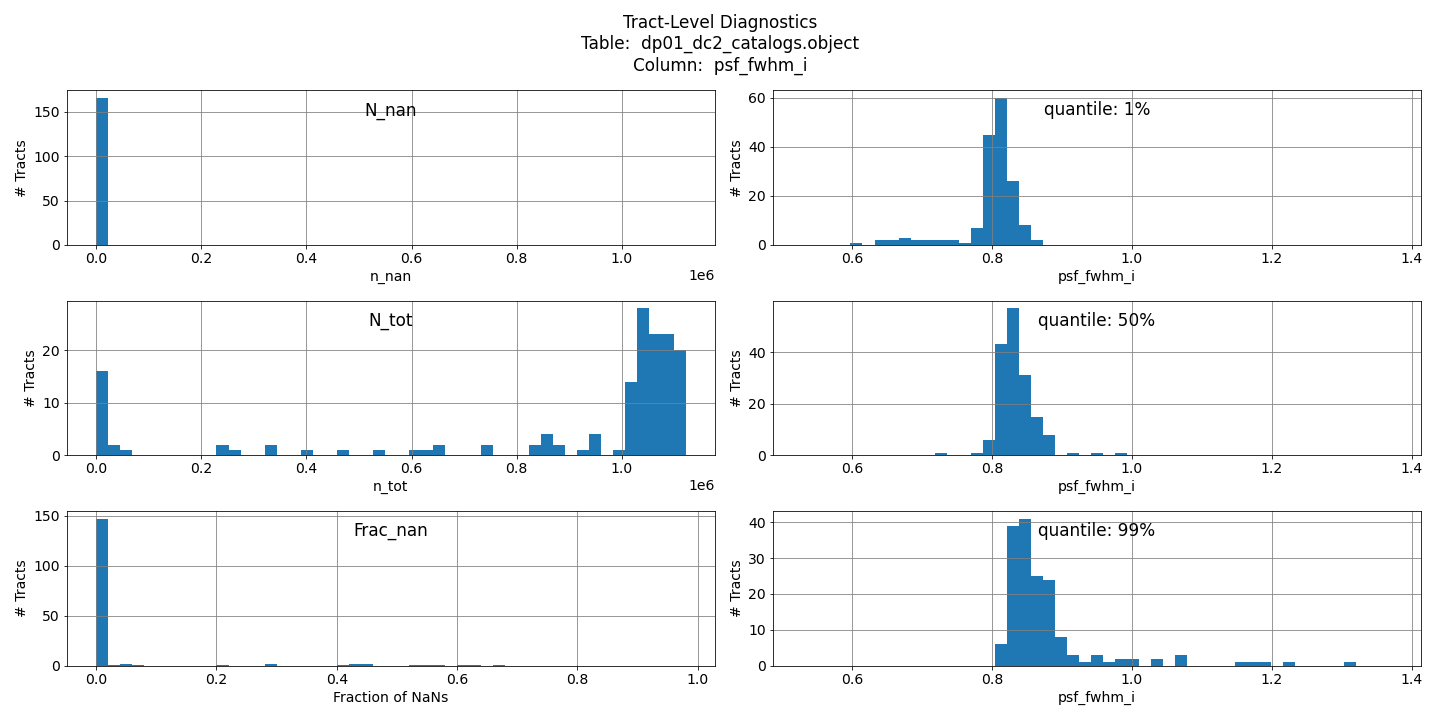
\includegraphics[width=1.0\linewidth]{Plots/TAP_verify_DP01.dp01_dc2_catalogs.object.psf_fwhm_i.png}
\caption{}
\label{fig:object_mag_i}
\end{figure*}



%TAP_verify_DP01.dp01_dc2_catalogs.object.mag_i.png
%TAP_verify_DP01.dp01_dc2_catalogs.object.magerr_i.png
%TAP_verify_DP01.dp01_dc2_catalogs.object.psf_fwhm_i.png


\subsection{\texttt{position} Table} \label{sec:position}



\subsection{\texttt{reference} Table} \label{sec:reference}



\subsection{\texttt{truth\_match} Table} \label{sec:truth_match}



\subsection{\texttt{forced\_photometry} Table} \label{sec:forced_photometry}



\section{Conclusions} \label{sec:conclusions}




\appendix
% Include all the relevant bib files.
% https://lsst-texmf.lsst.io/lsstdoc.html#bibliographies
\section{References} \label{sec:bib}
\renewcommand{\refname}{} % Suppress default Bibliography section
\bibliography{local,lsst,lsst-dm,refs_ads,refs,books}

% Make sure lsst-texmf/bin/generateAcronyms.py is in your path
\section{Acronyms} \label{sec:acronyms}
\addtocounter{table}{-1}
\begin{longtable}{p{0.145\textwidth}p{0.8\textwidth}}\hline
\textbf{Acronym} & \textbf{Description}  \\\hline

CPU & Central Processing Unit \\\hline
DESC & Dark Energy Science Collaboration \\\hline
DM & Data Management \\\hline
DP0 & Data Preview 0 \\\hline
DR2 & Data Release 2 \\\hline
IDF & Interim Data Facility \\\hline
LSST & Legacy Survey of Space and Time (formerly Large Synoptic Survey Telescope) \\\hline
RTN & Rubin Technical Note \\\hline
SQL & Structured Query Language \\\hline
TAP & Table Access Protocol \\\hline
deg & degree; unit of angle \\\hline
\end{longtable}

% If you want glossary uncomment below -- comment out the two lines above
%\printglossaries






\end{document}
